Lo primero que comprobamos del dataset es su gran tamaño, hay un total de 296021 muestras con 208 atributos cada una. Por lo que queda claro que vamos a proceder a reducir el dataset en la medida de lo posible.\\

Vamos a proceder a eliminar el atributo \textbf{appearedLocalTime}, la eliminamos en primer lugar por la dificultad de trabajar con este dato, el cual podríamos transformar en una serie de variables que desglosasen su contenido, no obstante tenemos otros atributos que ya lo hacen, como son la hora, el día, el mes y el año del avistamiento. Por otro lado vamos a eliminar también el atributo \textbf{X\_id} que como ya hemos comentado no sabemos qué representa. Además, teniendo en cuenta que la aplicación se lanzó el día 6 de julio de 2016, es claro que el año del avistamiento no aporta ninguna información, con lo que también eliminaremos el atributo \textbf{appearedYear}.\\

Viendo el dataset nos hemos dado cuenta de que para los atributos booleanos que nos indican si hay un gimnasio o una pokeparada a una distancia determinada del lugar de avistamiento del pokemon, siguen un patrón, y es que, al parecer, estas variables lo que indican es si hay un gimnasio o una pokeparada en un radio de una determinada longitud, con lo cual en cuanto el atributo que indica si hay un gimnasio a una distancia es cierto, el resto de atributos que indican si hay un gimnasio a una distancia mayor también lo son. \\

Lo mismo sucede con las paradas. Entonces una vez hayamos confirmado esto, como la existencia de un gimnasio o una pokeparada en un radio determinado implica la existencia en un radio mayor, podremos eliminar, sin pérdida de información, todos estos atributos y quedarnos únicamente con los atributos \textbf{gymDistanceKm} y \textbf{pokestopDistanceKm}, que resumirían la información contenida en los otros atributos. Para tratar de comprobar esto hicimos uso de las reglas de asociación con el paquete \textbf{arules}.\\

Obtuvimos las distintas reglas de asociación de tamaño 2 sin atender al soporte, ya que no estamos interesados en saber cuántas veces se da una correspondencia entre dos hechos (el soporte de dicha regla), lo que queremos saber es que cuando se da un hecho, esto implica que se den los que suponemos que deberían darse (la confianza de las reglas encontradas). Las reglas de asociación encontradas prueban nuestras suposiciones. Dado esto, procedimos a eliminar los atributos. Como la confianza es del 100\%, no afecta haber usado el conjunto entero para obtener dichas reglas.\\

Este dataset nos proporciona una serie de atributos para la localización del pokemon. Los primeros que nos encontramos son \textbf{latitude} y \textbf{longitude}, se tratan de coordenadas geográficas. Por otro lado aparecen \textbf{cellId\_90m}, \textbf{cellId\_180m}, \textbf{cellId\_370m}, \textbf{cellId\_730m}, \textbf{cellId\_1460m}, \textbf{cellId\_2920m}, \textbf{cellId\_5850m}.\\

Estos indican la posición geográfica usando celdas s2. Estas celdas se clasifican en niveles atendiendo a su área, desde 0 (menor área) a 30 (mayor área). Se obtienen según la longitud y la latitud, por lo que nos dan la misma información representada de distinta manera. Además, para métodos que dependen de una distancia como el KNN, tendríamos que investigar la distancia entre las distintas celdas a través de su ID, lo que supondría una carga de trabajo extra e innecesaria.\\

Se puede consultar más información sobre las celdas s2 en el siguiente \href{http://blog.christianperone.com/2015/08/googles-s2-geometry-on-the-sphere-cells-and-hilbert-curve/}{enlace}.\\

Por lo que acabamos de comentar se optó por eliminar los atributos correspondientes a las celdas, dejando los atributos \textbf{latitude} y \textbf{longitude} como los únicos para determinar la posición.\\

Una vez que limpiamos el dataset, añadimos información que nos resultó útil de cara a realizar clasificación y asociación.\\

Esta información son los \textbf{tipos} asociados a cada pokemon, pudiendo ser: agua, fuego, planta, hielo... y el \textbf{nombre} propio de cada pokemon, este último es equivalente a la clase del pokemon pero resulta más cómodo para realizar algunas interpretaciones.\\

Como ya hemos dicho en nuestro dataset tenemos información que nos permite conocer la posición en la que se produjo un avistamiento. Sin embargo, cuando pintamos los avistamientos que tenían como ciudad Madrid en el atributo city nos encontramos lo siguiente:

\begin{figure}[H] %con el [H] le obligamos a situar aquí la figura
\centering
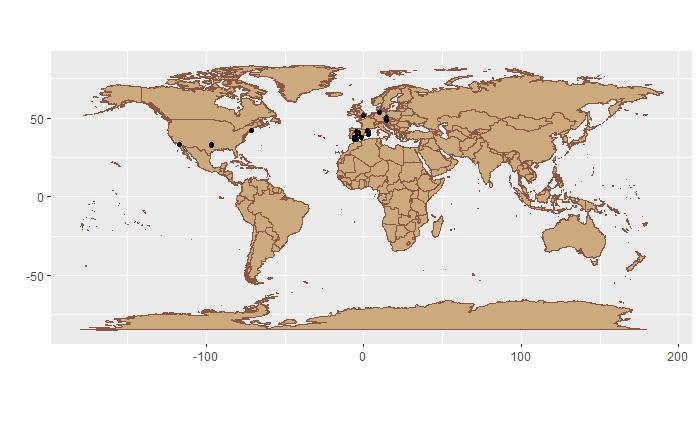
\includegraphics[scale=0.8]{img/madrid.jpg}  %el parámetro scale permite agrandar o achicar la imagen. En el nombre de archivo puede especificar directorios
\label{img/madrid.jpg}
\caption{Avistamientos Madrid}
\end{figure}

Es decir hay puntos en Madrid que no están situados en el mapa en una posición cercana a Madrid. En un principio pensamos que esto se debía a que el sistema de coordenadas del mapa sobre el que dibujamos los puntos, y los de la longitud y la latitud de nuestro dataset no coincidían. Pero antes de tomar una decisión sobre estos atributos decidimos dibujar los avistamientos relativos a pokemon que sólo aparecen en una regiones exclusivas: Mr. Mime en Europa, Tauros en Norte América, Kangaskhan en Australasia y Farfetch'd en Asia:

\begin{figure}[H] %con el [H] le obligamos a situar aquí la figura
\centering
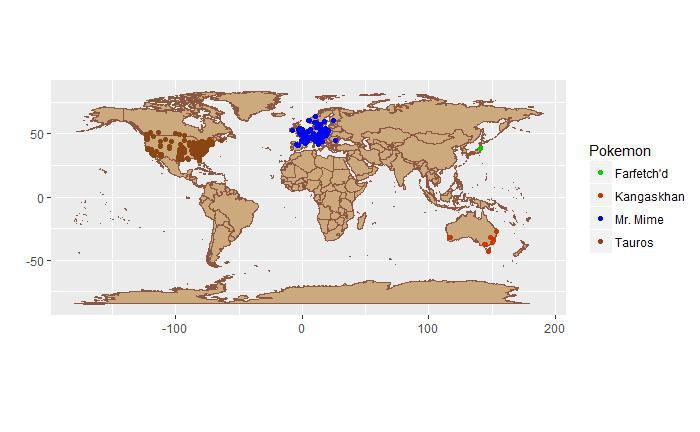
\includegraphics[scale=0.8]{img/exclusivos.jpg}  %el parámetro scale permite agrandar o achicar la imagen. En el nombre de archivo puede especificar directorios
\label{img/exclusivos.jpg}
\caption{Avistamientos regiones exclusivas}
\end{figure}

Como podemos ver la localización de estas visualizaciones es correcta, por lo tanto consideramos que las descripción del creador del dataset del atributo \textbf{city} no es correcta  \textbf\textit{the city of a sighting}. Así que o bien este atributo es la ciudad del usuario que vio el pokemon o el uso de proxys (que muchos usuarios emplearon para falsificar su posición y así poder acceder a pokemon de otras localizaciones distintas a la suya real) ha falseado los datos. En cualquiera de los casos esta información no es de utilidad para la predicción que queremos realizar, con lo que la eliminamos, junto con el atributo\textbf{continent}.\\

Pero antes tratas de darle una utilidad a esta información. Y es que un dataset no sirve únicamente para el problema que se plantea con él. Al tener datos de una aplicación empleada por tantos usuarios internacionalmente el número de datos indirectos que podemos extraer de él es muy grande, y de gran utilidad. En esta ocasión, considerando que el atributo \textbf{city} se refiere a la ciudad del usuario y que por tanto la localización de las observaciones se debe a viajes reales realizados por los usuarios, podemos extraer información sobre los desplazamientos realizados por los usuarios de la aplicación. Aquí vemos los viajes realizados por habitantes de Oslo:

\begin{figure}[H] %con el [H] le obligamos a situar aquí la figura
\centering
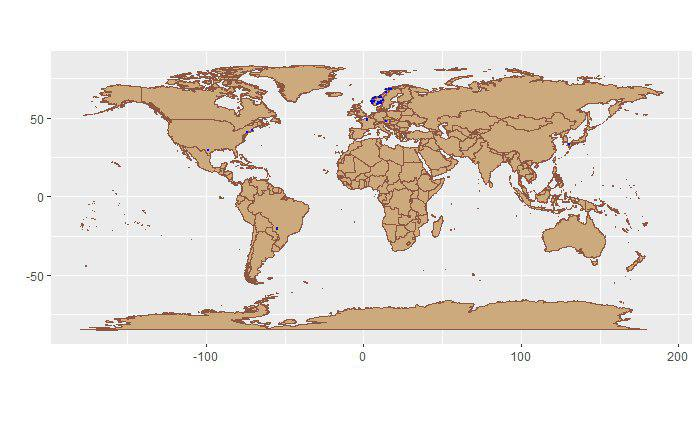
\includegraphics[scale=0.8]{img/oslo.jpg}  %el parámetro scale permite agrandar o achicar la imagen. En el nombre de archivo puede especificar directorios
\label{img/oslo.jpg}
\caption{Viajes realizados por los habitantes de Oslo}
\end{figure} 

En relación a estos datos indirectos que podemos obtener a partir de nuestro dataset podemos obtener también un mapa de temperaturas en el que se muestren las temperaturas en los lugares de los avistamientos. Como veremos más adelante los datos son relativos a una semana de agosto con lo que mostramos la temperatura referente a todos los avistamientos del dataset en un mismo mapa:

\begin{figure}[H] %con el [H] le obligamos a situar aquí la figura
\centering
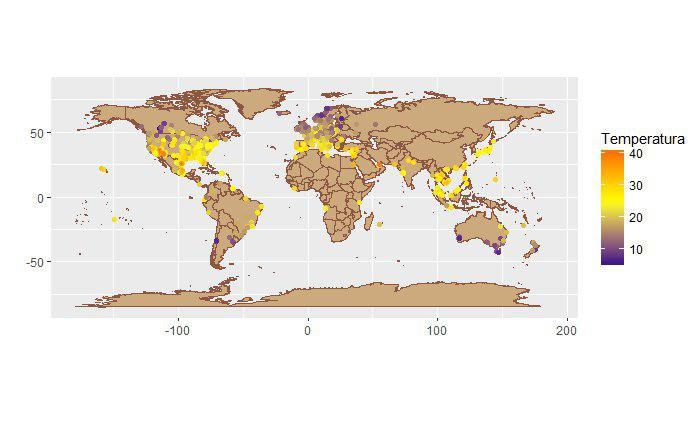
\includegraphics[scale=0.8]{img/temperatura.jpg}  %el parámetro scale permite agrandar o achicar la imagen. En el nombre de archivo puede especificar directorios
\label{img/temperatura.jpg}
\caption{Temperatura de los avistamientos}
\end{figure}

Aquí podemos apreciar por ejemplo como en Argentina las temperaturas son bajas en agosto, y como hay una diferencia de temperatura entre el norte y el sur de Europa.\\

Por otro lado al explorar el dataset observamos que en el atributo \textbf{appearedDayOfWeek} se tomaba el valor \textbf{dummy\_day}, y al consultar los valores que toma este atributo a lo largo del dataset vimos que no aparecía el lunes cuando el resto de los días de la semana sí que aparecen, con lo cual procedimos a revisar si este valor del atributo se corresponde con el lunes o es simplemente un valor perdido.\\

Observamos que el único día en el que se registran observaciones en las que el atributo toma el valor dummy\_day es el 8 de agosto, un lunes. Además, mientras se comprobaba este hecho observamos que todas las observaciones se realizaron en agosto y que además fue durante una semana de agosto, con lo cual el atributo \textbf{appearedMonth} no aporta ninguna información y además los atributos \textbf{appearedDayOfWeek} y \textbf{appearedDay} aportan la misma información, ya que al tomarse las muestras durante una sola semana hay una correspondencia biyectiva entre los valores de ambos atributos. Y como a priori no consideramos que la distancia entre días sea significativa, optamos por quedarnos con el atributo categórico.\\

Comprobamos también que podemos obtener los atributos sunriseMinutesMidnight y sunsetMinutesMidnight a partir de los atributos: \textbf{sunriseHour}, \textbf{sunriseMinute}, \textbf{sunsetHour} y \textbf{sunsetMinute}, con lo que procedemos a eliminar estos 4 últimos.\\

Veamos entonces cómo se distribuyen las muestras que tenemos según el tipo de pokemon avistado:

\begin{figure}[H] %con el [H] le obligamos a situar aquí la figura
\centering
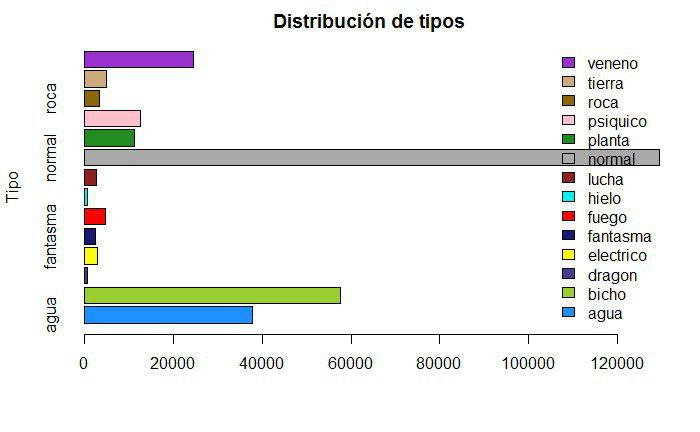
\includegraphics[scale=0.8]{img/tipos.jpg}  %el parámetro scale permite agrandar o achicar la imagen. En el nombre de archivo puede especificar directorios
\label{img/tipos.jpg}
\caption{Distribución de los tipos}
\end{figure}

Como podemos ver una vez que hemos agrupado las muestras por el tipo de pokemon, las clases están tremendamente desequilibradas. Mientras que hay muchísimos avistamientos de Pokemon de tipo normal, las clases hielo, dragón, fastasma, eléctrico o roca resultan marginales.\\

Creíamos que íbamos a apreciar una tendencia en la que los pokemon de tipo fantasma fuesen los que apareciesen con mayor frecuencia durante la noche, sin embargo todos los tipos siguen este patrón de aparición:

\begin{figure}[H] %con el [H] le obligamos a situar aquí la figura
\centering
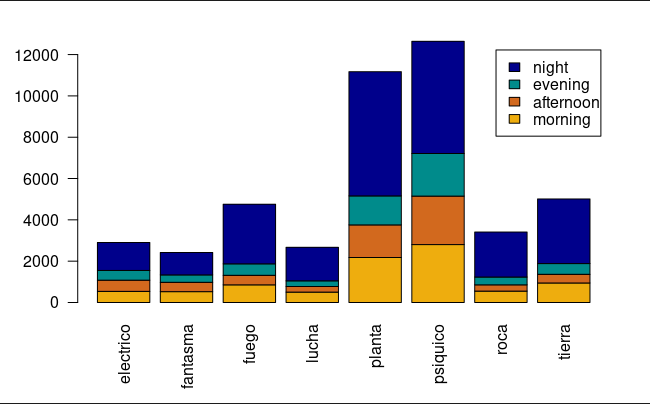
\includegraphics[scale=0.8]{img/noche1.png}  %el parámetro scale permite agrandar o achicar la imagen. En el nombre de archivo puede especificar directorios
\label{img/noche1.jpg}
\caption{Distribución de avistamientos a lo largo del día}
\end{figure}

\begin{figure}[H] %con el [H] le obligamos a situar aquí la figura
\centering
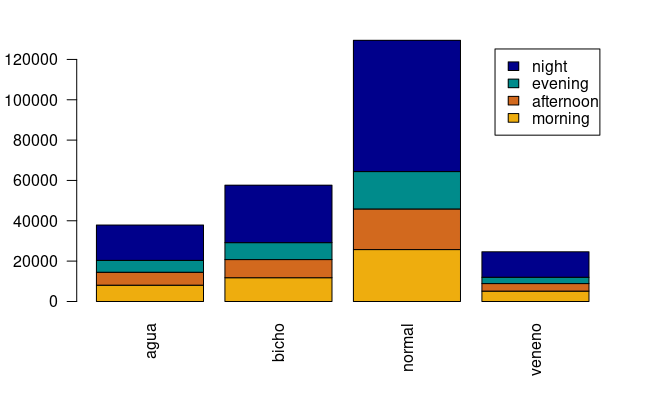
\includegraphics[scale=0.8]{img/noche2.png}  %el parámetro scale permite agrandar o achicar la imagen. En el nombre de archivo puede especificar dire2ctorios
\label{img/noche2.jpg}
\caption{Distribución de avistamientos a lo largo del día}
\end{figure}

\begin{figure}[H] %con el [H] le obligamos a situar aquí la figura
\centering
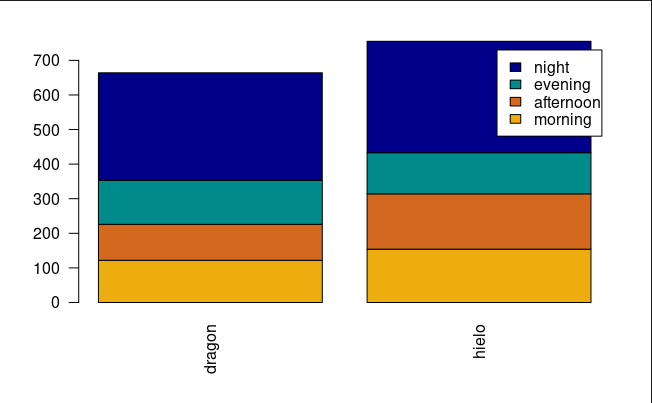
\includegraphics[scale=0.8]{img/noche3.png}  %el parámetro scale permite agrandar o achicar la imagen. En el nombre de archivo puede especificar directorios
\label{img/noche3.jpg}
\caption{Distribución de avistamientos a lo largo del día}
\end{figure}

Una de las principales características de Pokemon GO, aplicación de la cual son estos datos, es la posibilidad de encontrar pokemon en cualquier parte, por ejemplo en entornos cercanos al agua. Esperábamos, como es natural, que la mayoría de pokemon tipo agua se encuentren en zonas cercanas al agua. Esto daría un gran grado de realismo a la aplicación. Para comprobar esto generamos la siguiente gráfica:

\begin{figure}[H] %con el [H] le obligamos a situar aquí la figura
\centering
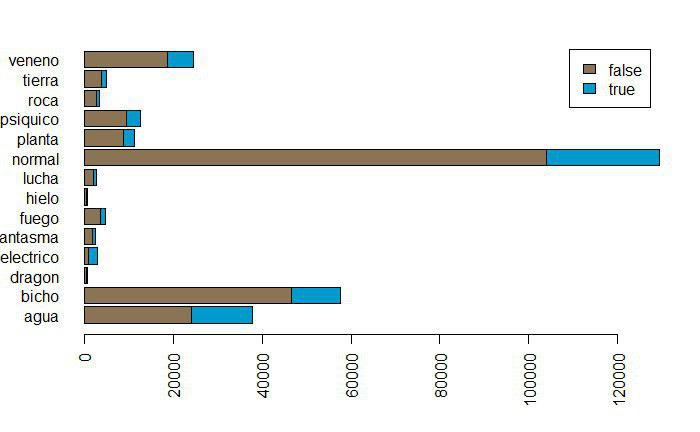
\includegraphics[scale=0.8]{img/cercaagua.jpg}  %el parámetro scale permite agrandar o achicar la imagen. En el nombre de archivo puede especificar directorios
\label{img/cercaagua.jpg}
\caption{Avistamientos cerca del agua}
\end{figure}

Así vimos que los pokemon de tipo eléctrico, dragón, agua e hielo son los que aparecen en mayor proporción cerca del agua. Por otro lado los pokemon de tipo fuego, planta, roca, normal y bicho son los que en menor proporción se presentan en zona acuosas (obtuvimos también una tabla para ver estos datos en cifras y no sólo visualmente). Nos sorprende de este análisis dos cosas: que no sean los pokemon de tipo agua los que sean más habituales en proporción en zonas acuosas y que los pokemon de tipo planta estén en menor proporción en las zonas con agua que en las zonas secas.\\

Aquí estamos hablando de proporciones, si nos fijamos en cantidades sí son los pokemon (después de los normales) de tipo agua los que aparecen más veces cerca del agua, no obstante preferimos atender a las proporciones ya que no queremos tener en cuenta que hay unos tipo de pokemon más difíciles de encontrar que otros.\\

Antes hemos estado discutiendo sobre los días de las apariciones de los diferentes pokemon. Por lo que ahora vamos a ver cómo se distribuyen dichas apariciones a lo largo de los días de la semana.

\begin{figure}[H] %con el [H] le obligamos a situar aquí la figura
\centering
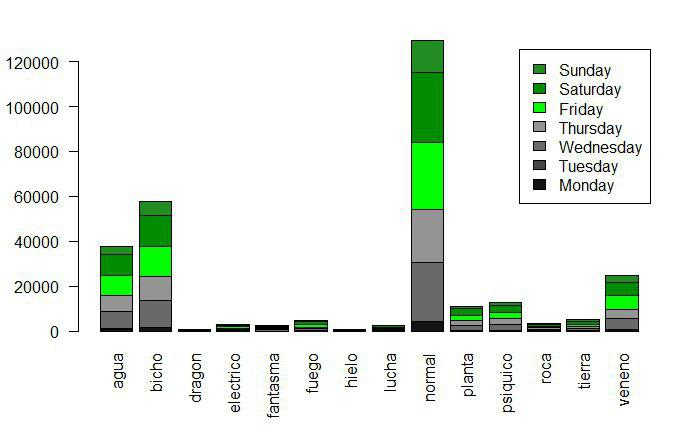
\includegraphics[scale=0.8]{img/semana.jpg}  %el parámetro scale permite agrandar o achicar la imagen. En el nombre de archivo puede especificar directorios
\label{img/semana.jpg}
\caption{Avistamientos a lo largo de la semana}
\end{figure}

Podemos observar que una gran parte de los avistamientos se realizan en el fin de semana, concretamente los sábados y viernes. También se producen una gran cantidad de avistamientos los miércoles y jueves, mientras que el lunes es el día que menos avistamientos se producen. Todo puede tener sentido, hemos de pensar que los datos que estamos tratando son de un vídeo juego para móviles, por lo tanto la mayor actividad, avistamientos, se realizará cuando los jugadores dispongan de mayor tiempo libre para jugar, fin de semana.\\

Ahora vamos a ver cómo se distribuyen los tipos de los distintos pokemon avistados en el mundo.

\begin{figure}[H] %con el [H] le obligamos a situar aquí la figura
\centering
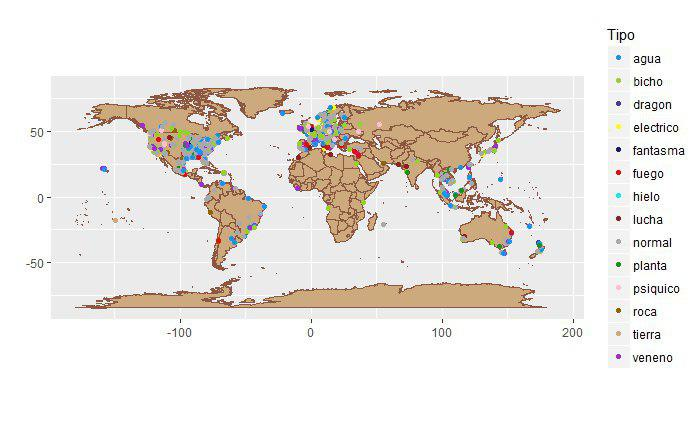
\includegraphics[scale=0.8]{img/tiposmundo.jpg}  %el parámetro scale permite agrandar o achicar la imagen. En el nombre de archivo puede especificar directorios
\label{img/tiposmundo.jpg}
\caption{Tipos de pokemon a lo largo del mundo}
\end{figure}

Podemos ver cómo no se sigue ningún tipo de distribución fija, no podemos obtener ningún tipo de patrón atendiendo a estos datos, por lo que se puede decir que los tipos de pokemon que aparecen son aleatorios.\\

Siguiendo esta línea estudiamos cómo se distrubuyen los tipos según la dirección e intensidad del viento:

\begin{figure}[H] %con el [H] le obligamos a situar aquí la figura
\centering
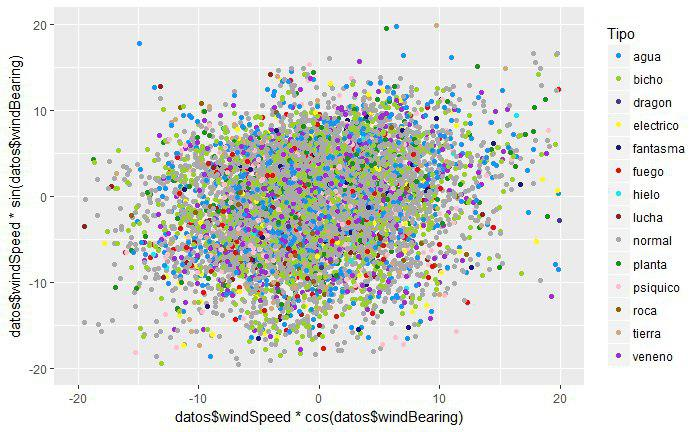
\includegraphics[scale=0.8]{img/viento.jpg}  %el parámetro scale permite agrandar o achicar la imagen. En el nombre de archivo puede especificar directorios
\label{img/viento.jpg}
\caption{Distribución de tipos según intensidad y dirección de viento}
\end{figure}

Aunque viendo los tipos uno por uno podríamos observar alguna tendencia hacia alguno de los cuadrantes de direcciones de viento lo cierto es que no hay una tendencia clara y podemos encontrar observaciones de cualquier tipo en cualquier dirección y velocidad, la densidad de puntos es mayor para velocidades menores pero para cualquier tipo se da la misma tónica. De hecho nos hemos restringido a una área más reducida para apreciar alguna tendencia y no hemos observado nada destacable.